\documentclass[9pt,a4paper,twocolumn]{scrartcl}
\usepackage{amssymb,amsmath,graphicx,fullpage,subfig,multirow}
\setkomafont{disposition}{\normalfont\bfseries}
\begin{document}

\title{The Kidney Transplant Process Model (KTPM)}
\subtitle{A Simulation Tool for the Transplant Process}
\subtitle{Masters Thesis}
\author{
    Christine Harvey \qquad Dr. Chia-Lin Wu\\
    Richard Stockton College of New Jersey\\
    Galloway, NJ\\
}
\date{}

\maketitle

\begin{abstract}
\textit {\textbf {Abstract}} - The Kidney Transplant Process Model (KTPM) was created to demonstrate the kidney transplant process from placement on the waiting list to life post-transplant.  The KTPM focuses on the effects of increased donor availability on the entire transplant process with a specific concentration on ethnicity.  The model was designed as a tool for analyzing the transplant process.  The model was built in Java using the MASON library for multi-agent simulations and supplemented with data from the Organ Procurement and Transplantation Network (OPTN) database and reports [1-3].
Experiments with this model have shown that if changes are not made to the kidney transplant process, the waiting list will continue to grow in the future.  While increases in the availability of donors will not eliminate the waiting list, these solutions could help to decrease the size of the list.  A specific increase in living donor transplants in minorities would also help to decrease the size of the waiting list for kidney transplants.
The KTPM is an effective and efficient way to model the waiting activity of the waiting list over time.  This model can be used to simulate and predict the effects of various changes to the current transplant system.
\end{abstract}

\section{Introduction}

There are currently over 95,000 people on the waiting list for a kidney transplant in the United States [1].  If the current transplant process continues as-is, this number of waiting patients will only continue to grow.  Even though the growth rate of active patients on the waiting list has slowed, it has been predicted that the waiting list will grow by over 4,000 people per year [4].
Patients are often placed on the kidney transplant waiting list after being diagnosed with End Stage Renal Disease (ESRD).  ESRD is permanent and occurs when the kidneys are no longer working well enough for a person to live without some form of treatment: dialysis or a transplant.  ESRD can be caused by either Acute or Chronic Renal Failure [5].  The two most commonly listed diagnoses for patients added to the waiting list in 2012 were Type II Diabetes and Hypertensive Nephrosclerosis [1].  A basic outline of the transplant process is shown in Fig. 1.
While waiting for a kidney transplant, patients undergo dialysis treatments which take over the kidney’s former job of filtering the bloodstream.  Dialysis is generally completed by patients at a facility three times a week for three to four hours at a time.  While this treatment allows patients to continue to live a relatively normal daily life, the quality of life for patients on dialysis is generally lower than patients that receive transplants [6].
Patients on the waiting list only need to continue dialysis until they have been selected to receive a transplant.  Having a transplant greatly increases the patient’s quality of life and patients can often resume a normal lifestyle.

\begin{figure}[h!]
  \caption{Simple outline of the transplant process.  Patients can transition between the stages of the process according to the directions on the chart.  The KTPM focuses on the transition between the dialysis and transplant stages as well as the post-transplant stage.}
  \centering
    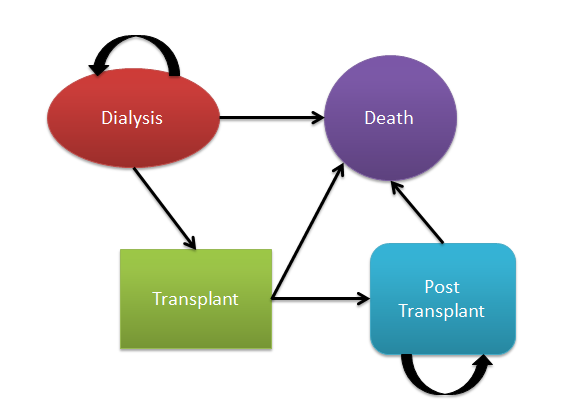
\includegraphics[width=0.5\textwidth]{Fig1}
\end{figure}

\begin{table*}[!ht] 
\caption{Waiting List Outcomes} % title of Table 
\centering % used for centering table 
\begin{tabular}{c c c| c c| c c} % centered columns (4 columns) 
\hline\hline \noalign{\smallskip}

& \multicolumn{2}{c|}{\textbf {Deceased Donor Transplant}} & \multicolumn{2}{c|}{\textbf {Living Donor Transplant}} & \multicolumn{2}{c}{\textbf {Other Removal Reason}}\\
\noalign{\smallskip}
\cline{2-7}
\noalign{\smallskip}
Ethnicity & Probablilty & Std. Error & Probablilty & Std. Error & Probablilty & Std. Error \\
\noalign{\smallskip}
\hline % inserts single horizontal line 
\noalign{\smallskip}
All Ethnicities & 10.91\% & 0.06\% & 5.21\% & 0.04\% & 7.54\% & 0.05\% \\
White & 12.90\% & 0.10\% & 9.28\% & 0.09\% & 9.01\% & 0.09\%  \\ 
African American & 10.41\% & 0.10\% & 2.22\% & 0.05\% & 6.98\% & 0.08\% \\
Hispanic/Latino & 8.56\% & 0.12\% & 4.03\% & 0.08\% & 6.37\% & 0.10\% \\
Asian & 9.72\% & 0.21\% & 3.30\% & 0.12\% & 5.79\% & 0.16\% \\
Other/Multi-Race & 8.80\% & 0.36\% & 3.08\% & 0.22\% & 7.33\% & 0.33\% \\

\noalign{\smallskip}
\hline %inserts single line 
\multicolumn{7}{l}{Note: Data collected from the OPTN Datebase records from years 2010-2012[1]}
\end{tabular} 
\label{table:outcomes} % is used to refer this table in the text 
\end{table*} 

\begin{table*}[!ht] 
\caption{Patient Survival Rates} % title of Table 
\centering % used for centering table 
\begin{tabular}{c c c c c| c c c c} % centered columns (4 columns) 
\hline\hline \noalign{\smallskip}

& \multicolumn{4}{c|}{\textbf {Deceased Donor Transplant}} & \multicolumn{4}{c}{\textbf {Living Donor Transplant}}\\
\noalign{\smallskip}
\cline{2-9}
\noalign{\smallskip}
Ethnicity & 3 Months & 1 Year & 5 Years & 10 Years & 3 Months & 1 Year & 5 Years & 10 Years \\
\noalign{\smallskip}
\hline % inserts single horizontal line 
\noalign{\smallskip}
All Ethnicities & 95.40\% & 91.20\% & 69.10\% & 41.80\% & 98.10\% & 96.40\% & 81.40\% & 58.90\% \\
White & 95.70\% & 91.50\% & 70.90\% & 44.80\% & 98.10\% & 96.30\% & 82.20\% & 60.20\% \\
African American & 94.20\% & 89.30\% & 62.20\% & 32.20\% & 97.70\% & 95.40\% & 73.20\% & 45.30\% \\
Hispanic/Latino & 95.90\% & 92.90\% & 75.00\% & 49.70\% & 97.90\% & 96.90\% & 84.80\% & 65.70\% \\
Asian & 96.80\% & 94.00\% & 76.30\% & 54.20\% & 99.00\% & 97.70\% & 88.90\% & 68.90\% \\
Other/Multi-Race & 97.10\% & 93.50\% & 75.30\% & 45.00\% & 99.30\% & 97.20\% & 81.20\% & 58.00\% \\
\noalign{\smallskip}
\hline %inserts single line 
\multicolumn{7}{l}{Note: Data collected from the 2009 OPTN Annual Report [2]}
\end{tabular} 
\label{table:survival} % is used to refer this table in the text 
\end{table*} 

\section{Background}

Previous research and studies have realized that there are currently ethnic disparities in the access to transplants for minority patients.  Currently, the percentage of deceased donor transplants for African Americans, Asians and Hispanic/Latinos in the U.S. lag behind the respective proportions of whites.  In an ideal and fair kidney transplant system, there would be no disproportions [7].  This research also noted that the disparity in access to Deceased Donor transplants has been narrowing significantly for African American patients in recent years, but not for Asian and Hispanic patients [7].  
Another study done by Peters in 2012 determined that there is no existing racial difference in patients receiving a living donor organ [8].  Research by Clark and Hicks determined that the completion of pre-transplant evaluations on potential recipients may pose a greater barrier to transplants among women, the poor and minorities.  It is also stated that African American patients are less likely than whites to be placed on waiting lists and receive transplants [9].
There are also discrepancies in patient survival among different ethnicities.  A study at the University of Michigan conducted a comparison between the mortality of African American and other racial/ethnic groups for simultaneous pancreas and kidney transplantation.  This study found that African American patients were twice as likely to lose the graft due to rejection compared to non-African Americans [10].  An analysis of transplant survival focusing on whites, African Americans, Asians and Hispanics noted that Asian kidney recipients  have the highest graft survival rate of all observed ethnicities.  The five year survival rate for Hispanics and Asians demonstrates “superior patient survival”, compared to African Americans and whites [7].
Table I shows the probabilities of various reasons patients are removed from the waiting list.  This data was collected and then aggregated from the Organ Procurement and Transplantation Network (OPTN) database, considering years 2010 to 2012 [1].  

\begin{table*}[!ht] 
\caption{Transplant Probabilities by Age} % title of Table 
\centering % used for centering table 
\begin{tabular}{c c c c c| c c c c} % centered columns (4 columns) 
\hline\hline \noalign{\smallskip}

& \multicolumn{4}{c|}{\textbf {Deceased Donor Transplant}} & \multicolumn{4}{c}{\textbf {Living Donor Transplant}}\\
\noalign{\smallskip}
\cline{2-9}
\noalign{\smallskip}
Ethnicity & 18-34 & 35-49 & 50-64 & 65+  & 18-34 & 35-49 & 50-64 & 65+ \\
\noalign{\smallskip}
\hline % inserts single horizontal line 
\noalign{\smallskip}
White & 12.57\% & 12.82\% & 13.05\% & 12.81\% & 18.64\% & 12.08\% & 8.49 \% & 5.40\% \\
African American & 10.81\% & 10.32\% & 10.69\% & 9.60\% & 4.17\% & 2.62\% & 1.83\% & 1.23\% \\
Hispanic/Latino & 9.79\% & 8.64\% & 8.30\% & 8.23\% & 9.07\% & 4.92\% & 2.80\% & 2.13\% \\
Asian & 10.28\% & 10.62\% & 9.30\% & 9.40\% & 8.72\% & 4.86\% & 2.33\% & 1.62\% \\
Other/Multi-Race & 9.43\% & 8.33\% & 9.14\% & 8.40\% & 4.88\% & 4.28\% & 2.36\% & 1.89\% \\
\noalign{\smallskip}
\hline %inserts single line 
\multicolumn{7}{l}{Note: Data collected from the OPTN Datebase records from years 2010-2012[1]}
\end{tabular}
\label{table:ages} % is used to refer this table in the text 
\end{table*} 

Table I shows the probability of patients receiving a deceased donor transplant, a living donor transplant, or to pass away or become too ill to receive a transplant.  It can be seen that very large differences exist between whites and all other ethnicities (especially African Americans) particularly for receiving living donor transplants.  The listed probabilities with the added influence of patient age were used in the model to determine patient’s probable outcomes on the waiting list.
Table II contains data collected from the 2009 Annual Report of the U.S. Organ Procurement and Transplantation Network [2].  This data shows the survival rate for patients at three months, one year, five years and ten years post-transplant.  This supports the study by Fan et al. that Asians and Hispanic/Latinos have a superior survival rate compared to other ethnicities [7].  More information about data and statistics used in the model can be found in the appendix.
There have been many recent discussions and initiatives taken to counteract the realized discrepancies between ethnicities and to improve the overall transplant system.  The National Kidney Foundation has launched the End the Wait campaign.  The goal of which is to increase the number of kidney transplants performed and completely eliminate the wait for organs within ten years.  This program includes focuses on improving the outcomes of first transplants, increasing deceased donor transplants and increasing living donor transplants [11]. 
It has been estimated that 10 to 12 thousand medically suitable people for organ donation die every year but only six thousand donate [12].  This knowledge, in combination with the potential for increased living kidney donation could significantly decrease the current waiting list.  One of the goals of this research is to study how increases in deceased and living donor transplant availability could affect the waiting list




\section{Methods}

The Kidney Transplant Process Model (KTPM) was built using data from the Organ Procurement and Transplantation Network (OPTN) Database.  This system was developed by UNOS and contains all data related to every organ donation and transplant event in the United States since October of 1987 [1].  Statistics taken from this database as well as from OPTN reports were used to generate and then validate the model [2].  
The model was created using MASON, a Java library core designed for discrete-event multi-agent simulations [3].  There are two forms of the model, a headless version to be used for parallel simulations as well as a GUI version that can be used to quickly execute and visualize single experiments.  

\subsection{Overview}
\subsubsection{Purpose}
The purpose of the Kidney Transplant Process Model (KTPM) is to demonstrate the kidney transplant process, from the initial waiting list to post-transplant survival.  In particular, this model focuses on the effects of increased organ availability on the entire transplant process.  Thousands of Americans die every year waiting for a transplant.  This model is a tool that can provide analysis for the effects of increased organ availability.  Increases in living and/or deceased donor transplants can be simulated and the resulting survival rated can then be analyzed.  This model includes a specific focus on patient age and ethnicity.

\subsubsection{Entities, state variables, and scales}
The KPTM is comprised of agents or patients that are experiencing the transplant process.  These agents can be divided into three collectives: patients on the waiting list, post-transplant patients, and deceased patients.  All patients have attributes that help determine their specific journey through the transplant process.  Every patient has an age and ethnicity.  As well as these characteristics each agent keeps track of how long they spend on the waiting list and how long they survive post-transplant.  For patients that have died, it is recoded how long they survived in addition to their cause of death (died waiting for a transplant or died post-transplant.)
The time step for the simulation is measured in one year increments.  Simulations are set to run for a ten year period.  At the end of the ten year time frame, all agents, living and deceased, are fully recorded for analysis.


\subsubsection{Process Overview and Scheduling}
The KTPM has several setup procedures that initialize the model and import all required probability matrices from external files.  These files contain the calculated probabilities obtained from the OPTN database.  The initial setup initially assigns all agents to be waiting for an organ transplant and assigns ethnicity and age to every agent according to the OPTN database probabilities.  Every new patient in the model is originally created with zero years recorded on the waiting list.  This version of the model excludes patients under the age of 18.  The available data for underage patients is considerably lower than all other age groups so the model was programmed to be able to run without this particular demographic.
After the initial setup has completed, the model runs over time steps that correspond to one year.  Each time step consists of the following four actions completed in the following order.
First, it is determined whether or not the agent will receive a transplant.  If the agent is currently on the waiting list, the Assign Transplant submodel will determine their next stage.  Agents can receive a living donor transplant, receive a deceased donor transplant, pass away while waiting for a transplant, be removed from the waiting list for another reason, or remain on the waiting list.  Patients that are removed from the waiting list for other reasons or that pass away are removed from the processes.  The agent’s passage through this submodel is determined using OTPN data based on the patient’s age and ethnicity.  
Next, the agents enter the Get Older submodel.  All living patients increase in age by one year.  This submodel includes a process for post-transplant patients that determines their odds of post-transplant survival.  This survival data comes from probabilities based on the agent’s type of transplant, number of years post-transplant and ethnicity. These probabilities are again based off the OTPN database.  In this submodel patients either survive the year or become deceased.  The post-transplant survival is only evaluated at certain years for which data exists. 
The third process in each time step is the addition of new patients to the waiting list.  A specified number of agents are added to the model and are initialized in the same process as the original waiting list patients in the model setup.  The number of agents added to the simulation is currently determined using the statistics of wait-list additions from previous years.  The assignment of ethnicity and age for these patients is determined using wait list additions probabilities from the OPTN database over the past three years.  
The final stage in each time step is the updating of global variables.  All information about the current state of the model is updated, including the percentage of transplanted patients, deceased patients, as well as the number of patients on the waiting list. 

\subsection{Design Concepts}
\subsubsection{Basic Principals}
The KTPM is based on the current United States organ waiting list and transplantation processes.  All data used in this model was gathered from the OPTN database.  The model has the ability to expand and extrapolate from the current state of the system using calculated probabilities for increased organ availability.  The increased organ availability is implemented in the Assign Transplant submodel.  
The model has the ability to provide insights to the transplant process by simulating the results stemming from improvements in organ availability.  The KTPM uses theories and ideas on increased organ availability stemming from previous research [7, 11]. 

\subsubsection{Emergence}
The model has two primary outputs.  The individual patient data is produced for every patient in each simulation.  This output can be aggregated to determine agent survival over time among different age and ethnic groups.  These results emerge from which patients receive transplants and how well each individual survives the process.  The second primary output is the overall statistics for each run.  This includes the final waiting list size, the number of surviving patients for each demographic and transplant type.  This data also emerges from the individual patient’s journey through the process.
The second form of output is particularly useful to determine and compare the effects or increased organ availability.  When multiple simulations have been completed with varying levels of increased organ availability for living and deceased transplants, these results can be analyzed and compared.

\subsubsection{Interaction}
Although the agents do not interact directly, the availability of resources affects the way the agents have access to organs.  The probability of an agent receiving a deceased donor transplant varies with the size of the waiting list.  Therefore if the waiting list decreases in size by more agents receiving transplants, the percentage of agents able to receive transplants will increase.

\subsubsection{Stochasticity}
Due to the probabilistic nature of the KTPM there are multiple instances of stochasticity implemented in the model.  Stochastic processes are used in the initial determination of agent’s age and ethnicity when adding agents to the model.  Randomly generated numbers are used to determine which demographic the agent is placed in.  Stochastic processes are also used in the Assign Transplant submodel to distinguish which patients receive transplants and which have alternative outcomes.  The final use of stochasticity in the model is the determination of agent survival post-transplant.  In all of these instances, a randomly generated number is used to establish which path the agent will follow.  These randomly generated numbers in accordance with the probabilities from the OPTN database determine the agent’s path in the process.

\subsubsection{Collectives}
This model contains three collectives, agents waiting for a transplant, agents that are post-transplant and deceased agents.  All agents begin the process waiting for a transplant.  The agent’s individual process determines which collective they transition to.  

\subsubsection{Observation}
The primary outputs of each individual simulation can be observed via the plots on the MASON interface.  The default visualization shows the size of the waiting list over time.  The second available graph displays the number of living donor transplants, deceased donor transplants, and the number of deaths each year.  Enhanced visualization for this simulation can be analyzed in a separate interface using details from the individual agent outcomes.
When multiple instances of the model are run in parallel, the final wait list size after the 15 year period can be visualized.  The outputs from the model can be accumulated and then displayed.  This display shows how the living and deceased factors affect the size of the wait list over the period of the simulation.
The other form of output, which is the overall simulation output with complete transplant numbers and survival outcomes can be compared and analyzed outside of the MASON interface across multiple simulation outputs.

\subsection{Details}
\subsubsection{Initalization}
The model can be initialized with any number of agents, in the GUI version of the model, the number of patients can be adjusted using the NumPatients box.  These agents are initialized in the model according to demographic probabilities from the OPTN database.  This model has been designed to run according to probabilities so all other initializations and calculations, such as the additions to the wait list are determined based on this initial number of patients.  For the experiments conducted in this research, 30 thousand patients are used as an initial input.
In addition to initializing the number of patients in the model, the living and deceased factor can be adjusted.  The values used for these parameters are listed in the experiments section of the paper for the individual experiments.  Generally, the deceased factor should be between 0.0 and 1.0, this range represents no increase to a 100\% increase in the number of available deceased donor kidneys.  The living factor can range from 0.0 to 2.0; this range represents no increase to a 200\% increase in the number of living kidney transplants.  The upper bound for this parameter can be higher than 2.0 if desired.   
Another parameter is the parameter to set up the model to equalize the probabilities of receiving a living donor transplant across ethnicities.  Setting this Boolean value to true sets all probabilities for living donor transplants as if the patient was of the white ethnicity.  By default this parameter is set to false.

\subsubsection{Input Data}
The KTPM includes a very large amount of input data.  The majority of this input data is statistics pulled from the OPTN database that determine agent demographics, probability of being taken off the waiting list as well as the survival probabilities for patients.  This data is all imported for each simulation from external files. 
The Living Factor and the Deceased factor are the two other forms of input data.  These two factors represent the increased availability of Organs.  The Living Factor determines the percent increase in Living Donor transplants, relative to the waiting list.  For example, a Living Factor of 50\% would correspond to a 50\% increase in living donor transplants on the waiting list.  The Deceased Factor determines the overall availability of Deceased Donor organs.  This number is not proportional to the size of the waiting list, as opposed to the Living Factor.  A Deceased Factor of 100\% would double the number of available deceased donor transplants overall.  Deceased Donor organ availability is unrelated to the size of the waiting list.  The same number of organs from deceased donors will be available, regardless of the size of the waiting list.

\subsubsection{Submodels}
The KTPM consists of two major submodels: Assign Transplant and Get Older.
The Assign Transplant submodel determines the next phase for the agent.  This submodel takes into account the agent’s age and ethnicity and then determines the probabilities for each possible outcome.  The possible outcomes include: Living Donor transplant, Deceased Donor transplant, death, removal from the waiting list for another reason, or remaining on the waiting list.  Each of these probabilities was pulled from the imported OPTN data.  The particular set of data for this submodel came from the waiting list removal report of candidates from 2010 to 2012 [1].  The Living and Deceased Donor transplants can be affected if the model is run with a Living or Deceased Factor.  If one or both of these factors are used, the corresponding probability will be increased as necessary.
If a patient receives a Living or Deceased Donor transplant they are marked as having received a transplant as with the specific type of transplant.  Patients that pass away while waiting for a transplant are removed from the waiting list and listed as deceased.  These patients are also recorded in the complete patient log written for every simulation.  This probability was composed of data gathered from the waiting list removal report with removal reasons listed as “Died” or “Too sick to transplant [1].  It was assumed that if a patient was removed from the waiting list because they were too ill to transplant, they would not recover.  
A final outcome of patients that result from this submodel are patients that were removed from the list for other reasons.  The reasons listed in the removal report include: “Transplanted in another country”, “Unable to contact candidate”, “Refused Transplant” as well as other various reasons.  These patients were completely removed from the simulation and recorded in the report as having left for “Other” reasons [1].
Living patients all experience the Get Older submodel.  This submodel begins by aging all of the agents by one year.  This submodel then splits into two paths, one for wait listed patients and one for transplanted patients.  The patients still on the waiting list simply have one more year added to their recorded number of years on the wait list.  The post-transplant patients experience a much more complex process.
Post-transplant patients need to be evaluated for survival at certain times.  Data is only available for post-transplant survival at three months, one year, five years and ten years [2].  This post-transplant survival data is from the 2009 Annual Report of the U.S. Organ Procurement and Transplantation Network [2].  Due to this specific data availability, patient’s post-transplant survival is evaluated at the post-transplant years of zero, one, five and ten.  In the other years, no survival evaluation is completed.  
If the agent is in one of the post-transplant evaluation years, their specific transplant survival probability, based on their ethnicity and number of years post-transplant, is used to determine their survival.  Different survival probabilities exist for Living and Deceased Donor transplant patients.  If a patient does not survive, they are marked as deceased and recorded in the complete patient log.  Patients that do survive the evaluation have one year added to their post-transplant years and continue on in the simulation.  
There is a special case for post-transplant patients, since there is a lack of data for patient survival for more than ten years.  Once a patient reaches eleven post-transplant years they are removed from the simulation and recorded as “Over 10 Year Survival” patients.  



\section{Experiments}

Three sets of experiments were run for this model.  The first set of experiments consisted of four basic runs of the model to determine the general effects of adjusting the Living and Deceased factors for the model.  The parameters for these experiments are outlined in Table IV.  Each of these trials for the experiments focused on trying to decrease the size of the waiting list.  The results from these experiments can be seen in Fig. 4 through Fig. 7.

\begin{table}[ht] 
\caption{Experiment Parameters for Set I} % title of Table 
\centering % used for centering table 
\begin{tabular}{p{1.5cm} p{1cm} p{1cm} p{2cm}} % centered columns (4 columns) 
\hline\hline %inserts double horizontal lines 
Trial Number & Living Factor & Deceased Factor & Waiting List Effect \\ [0.5ex] % inserts table 
%heading 
\hline % inserts single horizontal line 
Trial I & 1.0 & 1.0 & 18\% Increase \\ % inserting body of the table 
Trial II & 1.0 & 2.0 & 33\% Decrease \\ 
Trial III & 2.0 & 1.0 & 2\% Decrease \\ 
Trial IV & 2.0 & 2.0 & 45\% Decrease \\ [1ex]
\hline %inserts single line 
\end{tabular} 
\label{table:nonlin} % is used to refer this table in the text 
\end{table} 


The second set of experiments involved taking a closer look at the effects of the Living and Deceased factors on the model.  These trials involved a run over a wide range of parameters which are detailed in Table V.  This set of experiments resulted in 231 trials.  The results for this particular set of experiments can be visualized in Fig. 8.  The complete set of output data from these trials can be seen in Appendix B.  The generation of the second set of experiments was facilitated with the MITRE Goal-Directed Simulation Framework [14].  With this framework a simple parameter sweep over the areas of interest was completed and the output data was aggregated into a MySQL database for easy review.  Both sets of experiments were run with an initial waiting list size of 30,000.
These particular parameters were chosen because according to the current research, these are options within a reasonable scope.  There is a finite upper limit on the availability of deceased donors due to the number of available suitable deceased donors.  A deceased factor of 2.0 corresponds to a 100\% increase in the availability of deceased donor kidneys.  This could be reasonably achieved if every medically suitable person  would become and organ donor [12].  There is not such a strict limit on the availability of living donors.  Living donor kidneys can come from family members, friends or anonymous donors.  Despite the absence of a strict limit on this portion, it is not necessarily reasonable to assume that adequet living donor transplants are feasible.  A living factor of 3.0 corresponds to a 200\% increase in living donors.
The third and final experiment focused on equality in living donation.  As noted earlier, there is a significant disparity between ethnicities in living donor transplants [7, 15].  This experiment looks into how the waiting list would be affected if all ethnicities had exactly equal opportunities to receive a living donor transplant.  This is implemented by making all ethnicities have the same probabilities as the white ethnicity of receiving a living donor transplant.  The white ethnicity was chosen because this group of people has the highest probability of recieving a living donor transplant.  The probabilities are still different for each age group, but all probabilities are changed to match those of the white ethnic group.

\begin{table}[ht] 
\caption{Experiment Parameters for Set II} % title of Table 
\centering % used for centering table 
\begin{tabular}{c c c c} % centered columns (4 columns) 
\hline\hline %inserts double horizontal lines 
Parameter & Min & Max & Step Size\\ [0.5ex] % inserts table 
%heading 
\hline % inserts single horizontal line 
Living Factor & 1.0 & 3.0 & 0.1 \\ 
Deceased Factor & 1.0 & 2.0 & 0.1  \\ [1ex]
\hline %inserts single line 
\end{tabular} 
\label{table:experiment2} % is used to refer this table in the text 
\end{table}

\section{Results}
\subsection{Experiment Set I}
The results from Experiment Set I show the effects of the living and deceased factors on the transplant process.  The results and parameters for this experiment are all displayed in Table IV.  The data from Trial I, shown in Fig. 4 shows that if nothing is done to improve the effectiveness of the transplant process, the waiting list will continue to grow.  This will lead to an increased number of patients that will die while waiting for a transplant.
Doubling the availability of deceased donor kidneys would have a very crucial impact on the waiting list for kidney transplants as seen in Fig. 5.  An increase in this field could decrease the size of the waiting list by 33\%.  Fig. 6 displays how the wait list will be affected if there is a 100\% increase in living donor transplants.  While there is not a significant decrease in the size of the waiting list, it is important to note that this change could stop the size of the list from increasing.  A 100\% increase of both living and deceased donors would have the largest impact on the waiting list as shown in Fig. 8.

\subsection{Experiment Set II}
The findings from the second experiment set provide a more detailed look into how the size of the waiting list could be affected if there were to be increases in the number of living and deceased donors.  The results from this experiment are visualized in Fig. 8.  This representation shows the living factor and the deceased factor respectively on the x and y axes.  The color of the point at each combination reflects the size of the wait list after 15 years.  The red points in the bottom left corner correspond to an increased waiting list and little increase in the living and deceased donor factors.  The points in the upper right corner represent the highest living and deceased factors as well as the largest decrease in the waiting list size.  A living factor of 2.0 along with a deceased factor of 1.0 could lead to a 52\% decrease in the size of the waiting list.

\begin{figure}[h!]
  \caption{Visualization created in Paraview to show the size of the list after 15 years when various living and deceased factors are used in the experiments.}
  \centering
    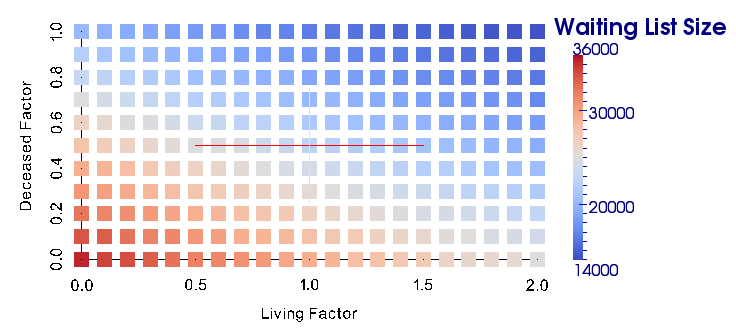
\includegraphics[width=0.5\textwidth]{MEGOut}
\end{figure}

\subsection{Experiment Set III}
The goal of the third experiment set was to explore the effects of equalizing the living transplant probabilities across all ethnic groups.  For this experiment, the probabilities to receive a living donor transplant were set based off of the patient’s age group and the white ethnic group.  This is an attempt to improve the vast differences in probabilities observed in Table III.  
Fig. 9 shows that if the probability of receiving a living donor transplant for all ethnicities was increased to match that of the white ethnicity, the wait list would decrease in size over the next 15 years.  This change would account for a 3.5\% decrease in the size of the waiting list.  While this might seem like a small percentage, this would correspond to over 3,000 people (CEH:per year or total???).

\section{Discussion}
The simulation results gathered from the model showed that an increase in donors is necessary to keep the transplant waiting list from growing.  These results are in agreement with the study by Leichtman, A.B., et al., that the size of the waiting list will continue to increase unless there is a change. 
The results from Experiment Set II showed that if there are significant increases in the number of deceased and living donors, the size of the waiting list will decrease.  Although, this model demonstrates that a decrease is feasible, the implementation of such dramatic changes to the current transplant system could be very difficult.  The previously mentioned End The Wait program proposes eliminating the entire waiting list in the next ten years [11].  The results from this model tend to disagree with the reality of this goal.  In the simulation, a 100\% increase in deceased donors and a 200\% increase in living donors only led to a 52\% reduction over 15 years.  While this outcome would be a significant improvement, the result is still very far from eliminating the wait list entirely in just ten years.
The outcomes observed from Experiment Set III show that improvements to the equality in living donor transplants could help decrease the transplant waiting list.  Even small measures taken to remove disparities between can help to stop the rapid growth of the transplant list and possibly reduce the size of the waiting list.
This model was created based on many assumptions.  The data used to create the model was based on recent years passed and does not account for improved medical technologies or improvements in the scope of the model.  Therefore, the model assumes that organs will continue to be distributed in the same manner.  
The model also assumes that patients will be added and removed from the waiting list in the same pattern observed between 2010 to 2012.  This disregards general improvements in kidney health in the future.  The KTPM also does not account for surviving failed transplant patients.  Patients can survive failed transplant surgeries and be added back to the waiting list [1].
Many of these items that were not considered in this version of the model could be implemented in the future.  
VII.	CONCLUSIONS
The KTPM can be used to simulate the entire kidney transplant process.  Results from experiments generated with this model can be used to investigate potential changes to the process.  It could be useful to see how changes to living and deceased donors as well as changes to donor ethnicity could affect the entire process.  The model’s setup by ethnicity and age also makes it a valuable tool to investigate the differences in these areas in the transplant process.  There are many interesting disparities between ethnicities in the transplant process that can be examined with this model.
There is an abundance of potential future work with this model.  There are many appealing areas of the transplant process for every organ that can be explored with an expanded version of this model.  A particular area of interest that this model is suitable for would be an analysis of the effects of increased donor availability on patient survival.  
In conclusion, it has been shown that a computational model can be used to explore the effects of various hypothetical changes to the transplant process. This model has also shown that alterations must be made to the transplant process before the size of the waiting list becomes unmanageable.

\section{Acknowledgement}
We thank Dr. Russell Manson, Dr. Robert Olsen, Dr. Monir Sharobeam, and Dr. William Baldwin from The Richard Stockton College of New Jersey for their guidance and support. MITRE???


\begin{thebibliography}{1}
	\bibitem{hrsa} Health Resources and Services Administration, Data. 2013  [cited 2013 March 30]; Available from: http://optn.transplant.hrsa.gov/data/.
    \bibitem{hhs} U.S. Department of Health and Human Services, 2009 Annual Report of the U.S. Organ Procurement and Transplantation Network and the Scientific Registry of Transplant Recipients: Transplant Data 1999-2008. . 2009, Health Resources and Services Administration, Healthcare Systems Bureau, Division of Transplantation: Rockville, MD.
    \bibitem{mason}	[3]	Luke, S., et al., MASON: A Multiagent Simulation Environment. SIMULATION, 2005. 81(7): p. 517-527.
    \bibitem{leichtman} Leichtman, A.B., et al., Kidney and pancreas transplantation in the United States, 1997-2006: the HRSA Breakthrough Collaboratives and the 58 DSA Challenge. Am J Transplant, 2008. 8(4 Pt 2): p. 946-57.
    \bibitem{ESRD} American Kidney Fund, End Stage Renal Disease (ESRD). 2008  [cited 2013 April 14]; Available from: http://www.kidneyfund.org/kidney-health/kidney-failure/end-stage-renal-disease.html.
    \bibitem{evans} Evans, R.W., et al., The quality of life of patients with end-stage renal disease. The New England Journal of Medicine, 1985. 312(9): p. 553-559.
    \bibitem{fan} Fan, P.Y., et al., Access and Outcomes Among Minority Transplant Patients, 1999–2008, with a Focus on Determinants of Kidney Graft Survival. American Journal of Transplantation, 2010. 10(4): p. 1090-1107.
    \bibitem{peters} Peters, T.G., Good News Regarding Race and Kidney Transplant Access in America. American Journal of Transplantation, 2012. 12(4): p. 810-811.
    \bibitem{clark} Clark, C.R., et al., Promoting Access to Renal Transplantation: The Role of Social Support Networks in Completing Pre-transplant Evaluations. JGIM: Journal of General Internal Medicine, 2008. 23(8): p. 1187-1193.
	\bibitem{luan} Luan, F.L., et al., Influence of Recipient Race on the Outcome of Simultaneous Pancreas and Kidney Transplantation. American Journal of Transplantation, 2010. 10(9): p. 2074-2081.
	\bibitem{nkf} National Kidney Fondation, Inc. End The Wait! 2013  [cited 2013 March 4]; Available from: http://www.kidney.org/transplantation/endthewait/index.cfm.
	\bibitem{etzioni} Etzioni, A., Organ Donation: A Communitarian Approach. Kennedy Institute of Ethics Journal, 2003. 13(1): p. 18.
	\bibitem{grimm} Grimm, V., et al., The ODD protocol: A review and first update. Ecological Modeling, 2010. 221(23): p. 8.
	\bibitem{page} Page, E.H., et al. Goal-Directed Grid-Enabled Computing for Legacy Simulations. in Cluster, Cloud and Grid Computing (CCGrid), 2012 12th IEEE/ACM International Symposium on. 2012. IEEE.
	\bibitem{kierans} Kierans, C. and J. Cooper, Organ donation, genetics, race and culture: The making of a medical problem. Anthropology Today, 2011. 27(6): p. 11-14.G. Eason, B. Noble, and I. N. Sneddon, “On certain integrals of Lipschitz-Hankel type involving products of Bessel functions,” Phil. Trans. Roy. Soc. London, vol. A247, pp. 529–551, April 1955.

\end{thebibliography}

\end{document}